\subsubsection{UC31 - Visualizzazione errore nome dizionario dati}\label{UC31}

\begin{figure}[H]
  \centering
  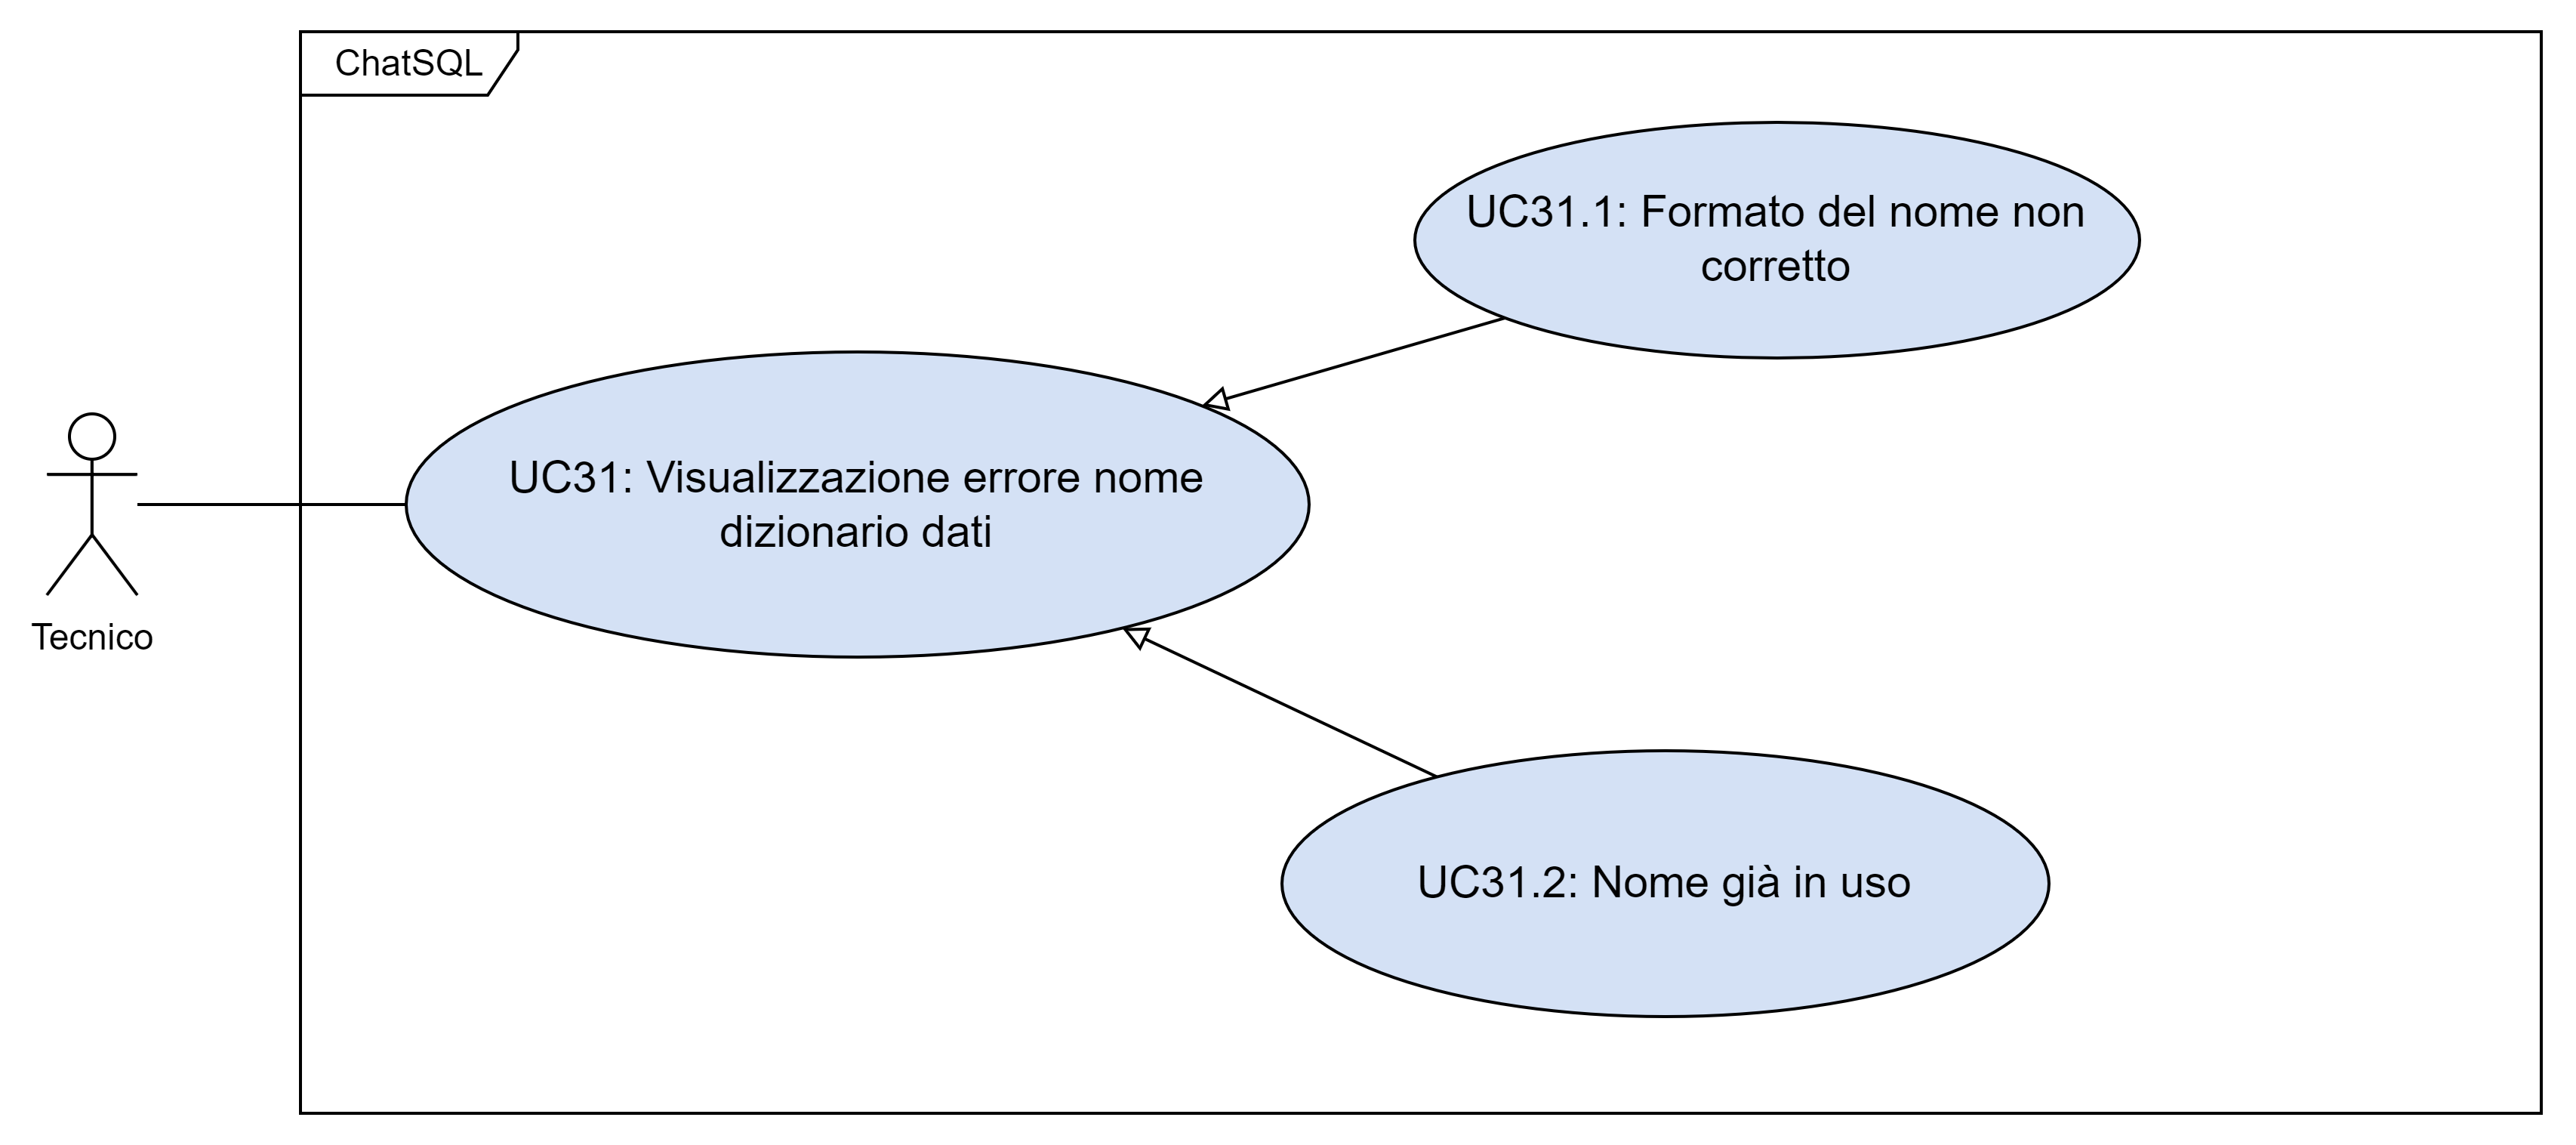
\includegraphics[width=0.90\textwidth]{assets/uc31.png}
  \caption{UC31}
\end{figure}

\paragraph*{Descrizione}
Nel caso cui il sistema riscontri delle anomalie nella validazione del nome di un \glossario{dizionario dati}, il Tecnico visualizza un messaggio d'errore.

\paragraph*{Attori principali}
Tecnico

\paragraph*{Precondizioni}
\begin{itemize}
  \item Il Tecnico ha richiesto l'inserimento o la modifica di un \glossario{dizionario dati} nel sistema;
  \item Il nome del dizionario dati non è valido.
\end{itemize}

\paragraph*{Postcondizioni}
\begin{itemize}
  \item Viene visualizzato un messaggio d'errore esplicativo;
  \item L'operazione di salvataggio o modifica non viene portata a termine.
\end{itemize}

\paragraph*{Scenario principale}
\begin{enumerate}
  \item Il sistema riscontra un errore nella validazione del nome di un \glossario{dizionario dati};
  \item Il sistema restituisce un messaggio con i dettagli dell'errore.  
\end{enumerate}

\paragraph*{Specializzazioni}
\begin{itemize}
  \item Formato del nome non corretto (\hyperref[UC31point1]{UC31.1});
  \item Nome già in uso (\hyperref[UC31point2]{UC31.2}).
\end{itemize}

%%%%%%%%%%%%%%%%%%%%%%%%%%%%%%%%%%%%%%%%%%%%%%%%%%%%%%%%%%%%%%%%%%%%%%%%%%%%%%

\subsubsection{UC31.1 - Formato del nome non corretto}\label{UC31point1}
\paragraph*{Descrizione}
Il sistema restituisce un messaggio di errore nel caso in cui il formato del nome sia invalido.

\paragraph*{Attori principali}
Tecnico

\paragraph*{Precondizioni}
\begin{itemize}
  \item Il formato del nome di un \glossario{dizionario dati} è errato.
\end{itemize}

\paragraph*{Postcondizioni}
\begin{itemize}
  \item Viene restituito un messaggio d'errore esplicativo.
\end{itemize}

\paragraph*{Scenario principale}
\begin{enumerate}
  \item Il sistema riscontra un errore nella validazione del nome;
  \item Il sistema restituisce un messaggio con i dettagli dell'errore.  
\end{enumerate}

%%%%%%%%%%%%%%%%%%%%%%%%%%%%%%%%%%%%%%%%%%%%%%%%%%%%%%%%%%%%%%%%%%%%%%%%%%%%%%

\subsubsection{UC31.2 - Nome già in uso}\label{UC31point2}
\paragraph*{Descrizione}
Il sistema restituisce un messaggio di errore nel caso in cui il nome di un \glossario{dizionario dati} non sia univoco.

\paragraph*{Attori principali}
Tecnico

\paragraph*{Precondizioni}
\begin{itemize}
  \item Nel sistema è già presente un \glossario{dizionario dati} con lo stesso nome.
\end{itemize}

\paragraph*{Postcondizioni}
\begin{itemize}
  \item Viene restituito un messaggio d'errore esplicativo.
\end{itemize}

\paragraph*{Scenario principale}
\begin{enumerate}
  \item Il sistema riscontra un errore nella validazione del nome;
  \item Il sistema restituisce un messaggio con i dettagli dell'errore.  
\end{enumerate}
